\chapter{音声波形と内容の2面から行う偽情報の検出}\label{ch:spc_cnt}
%TODO: 発話内容を考慮した→音声波形の内容の2面から行う
\section{目的}\label{sec:cnt_pur}
%TODO: 話者照合云々は関連研究へ
% \subsection{形式の位置づけ}
% 音声を入力とする話者認識(Speaker Recognition)には、話者識別(Speaker Identification)と話者照合(Speaker Verification)という2種類の形式がある \cite{FURUI1997859,628714,5745552}。
% \cref{fig:speaker_recog}は2種類の形式の違いを示す。

% \begin{figure}[h]
%     \centering
%     \begin{minipage}{0.9\linewidth}
%         \centering
%         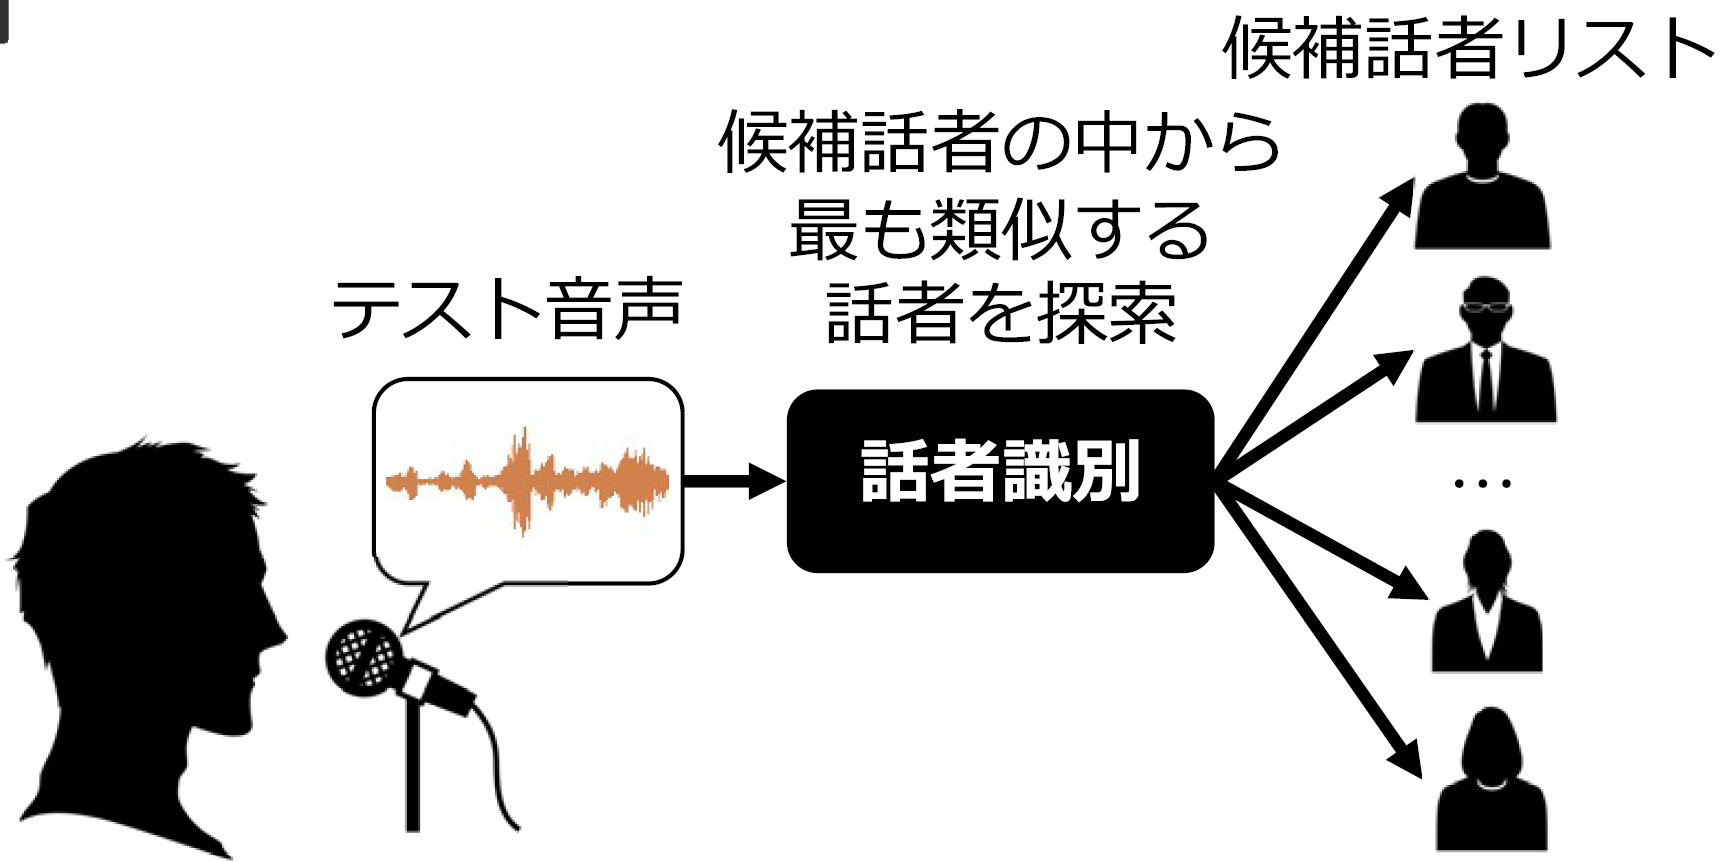
\includegraphics[width=0.8\linewidth]{figures/sd.png}
%         \subcaption{話者識別}
%     \end{minipage}
%     \begin{minipage}{0.9\linewidth}
%         \centering
%         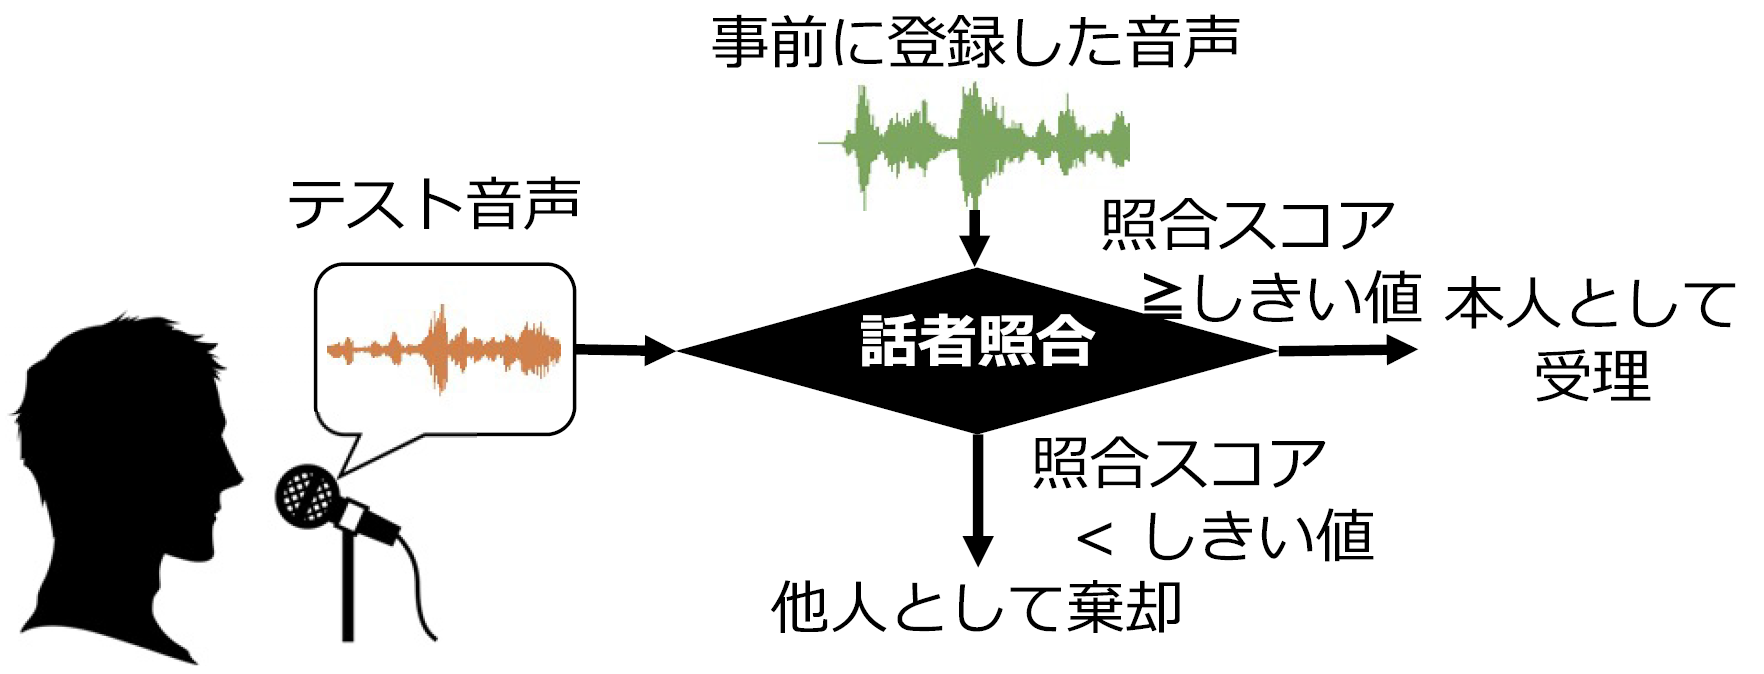
\includegraphics[width=0.8\linewidth]{figures/sv.png}
%         \subcaption{話者照合}
%     \end{minipage}
%     \caption{話者認識の形式 \cite{俵直弘2022}}
%     \label{fig:speaker_recog}
% \end{figure}

% 話者識別は事前に登録した複数の候補者の中から提示された音声の話者を探索する1対nの推定問題であるのに対し、
% 話者照合では,提示された二つの音声が同一話者によるものか否かを推定する1対1の照合問題として定義する \cite{俵直弘2022}。
% 識別では、未知の話者を既知の話者のデータベースと比較し、最もよく一致する話者を識別結果として与える。
% 一方で照合では、音声サンプルが主張された人物によって話されたかどうかを判断するタスクと言える \cite{1561284}。
% よって、本研究で行うなりすまし偽音声の検出は、話者照合に該当する。

% また,話者認識は,登録時と照合時で同じ内容の音声を用いるテキスト依存型(text-dependent)と,
% 登録時と照合時で異なる内容の音声を用いるテキスト独立型(text-independent)に分類される \cite{俵直弘2022}。
% ASVspoofにおけるなりすまし検出では、テキスト依存型の形式を取っている。
% 読み上げる音声は本人・偽いずれも新聞記事から引用した同一の文章を読み上げているため、
% 実際にSNS上で偽音声による偽情報が投稿された状況から乖離がある。
% よって本研究では、テキスト独立型の話者照合を行う。

\subsection{検出対象の位置付け}
本研究の目的は、偽情報を話すなりすまし音声(偽音声)を自動で検出することである。
偽情報を話す偽音声には内容の確からしさと音声そのものの本人性という2種類の概念をもつ。
話す内容の確からしさは、事実か・偽情報かの2種がある。
本来ではこの2種類以外に事実ではないものの意図的に発信されたものではない誤情報もあるが、本章では考慮しない。
本人性は本人が話すか・本人以外がなりすましているかの2種がある。
本人以外がなりすます場合では機械による合成処理を含まない場合(声真似等)もあるが、
意図的に社会に不安を与える行為として行われにくいと考えられるため本章では考慮しない。

よって、偽情報を話すなりすまし音声を検出する場合、モデルへ入力する対象は内容の確からしさと本人性から以下の4種類が挙げられる。

\begin{itemize}
    \item 偽情報を話すなりすまし音声(検出したい対象)
    \item 事実を話すなりすまし音声
    \item 偽情報を話す本人音声
    \item 事実を話す本人音声
\end{itemize}

また、\cref{fig:twoPerspective}は内容信憑性・本人性の2次元で定義される、本研究の扱う音声の空間を表す。

\begin{figure}[h]
    \centering
    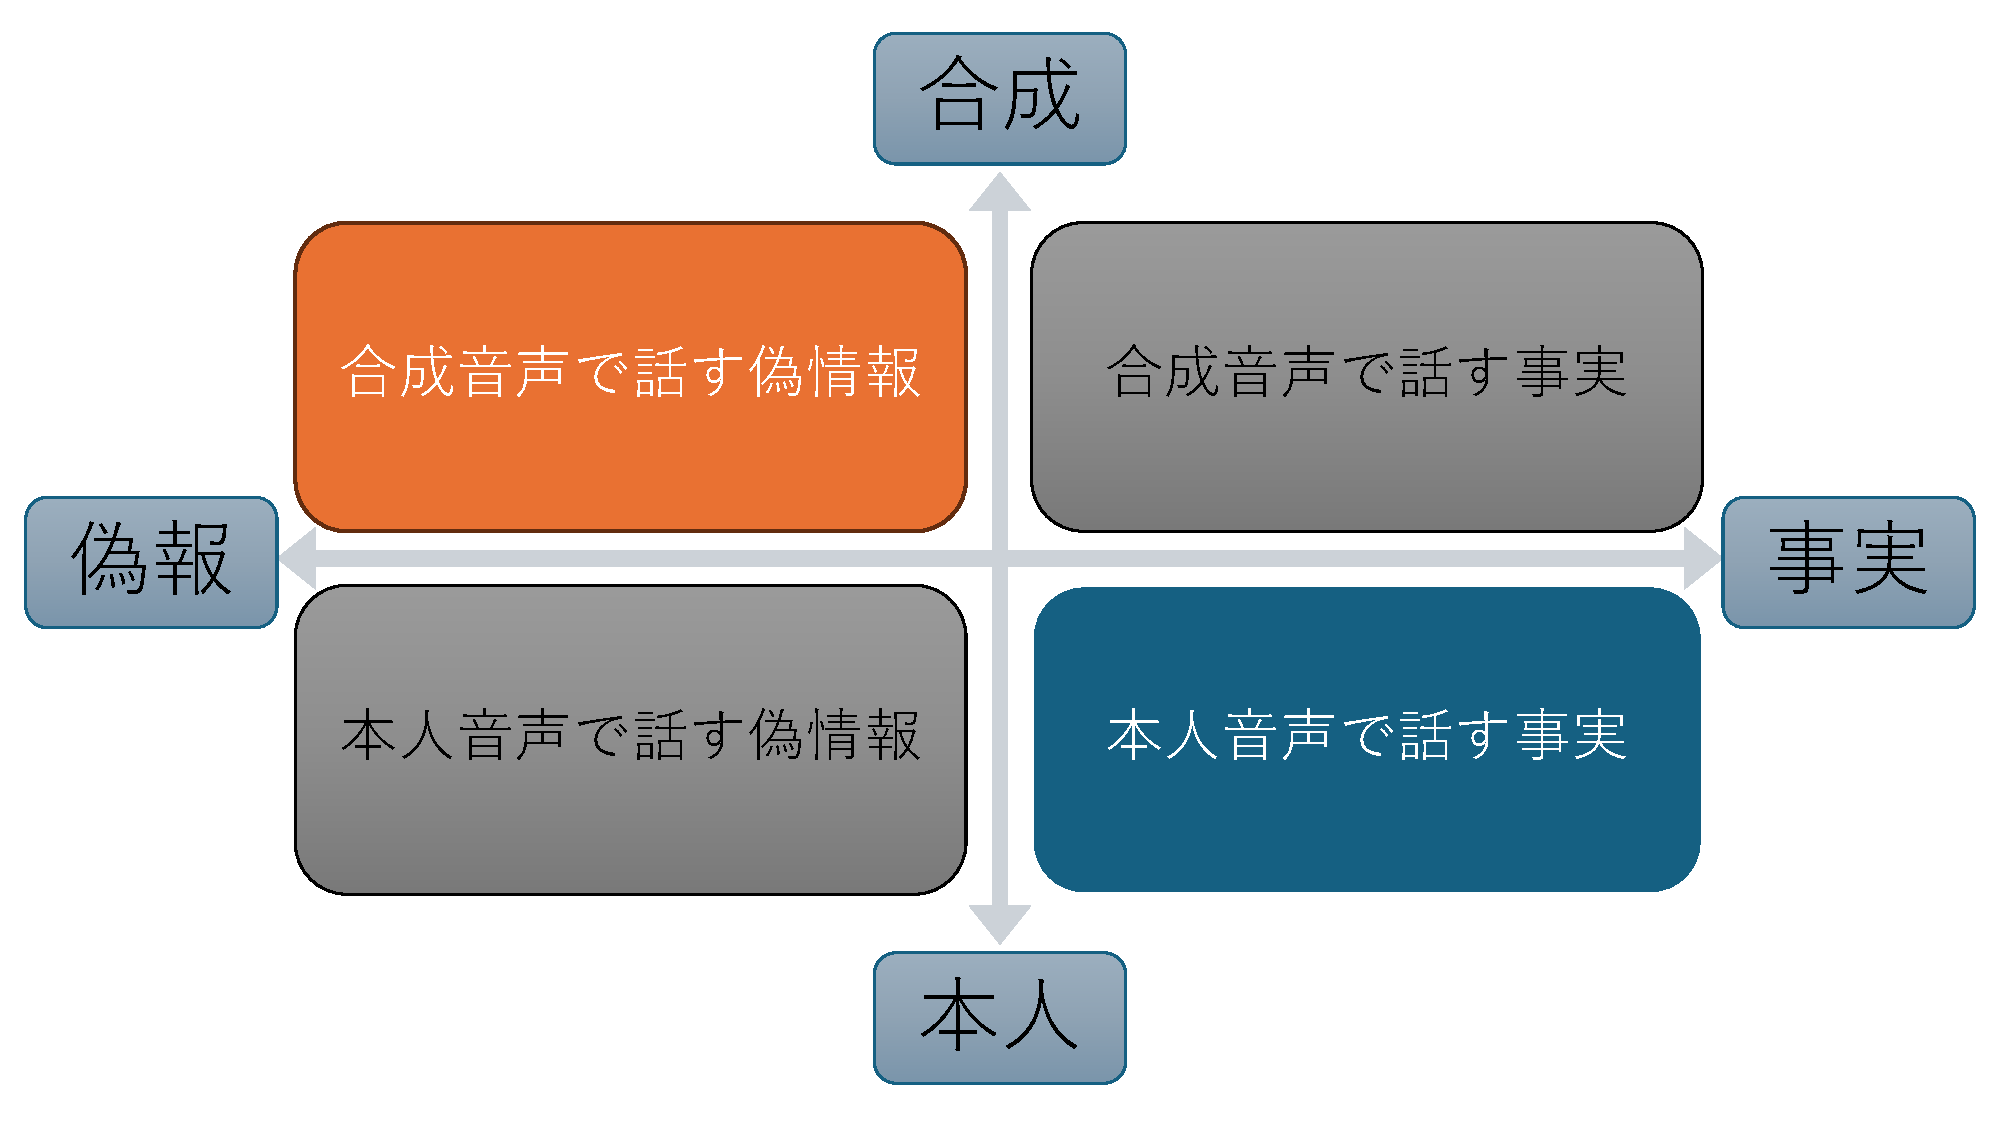
\includegraphics[width=\linewidth]{figures/D論概念図.pdf}
    \caption{発話内容の信憑性と、発話者の本人性による音声の種類。本研究では合成音声で話す偽情報と本人音声で話す事実の2種類に着目する。}
    \label{fig:twoPerspective}
\end{figure}

事実を話す本人音声は、偽情報を話すなりすまし音声とは
内容の信憑性及び本人性において、対極に位置する概念である。
本研究の予備実験では、既存手法が合成音声と本人音声を正しく識別できるかを調べるために、事実を話す本人音声を検出すべきでない対象とした。
%要確認

事実を話すなりすまし音声は、主にマスメディアによるニュース記事の読み上げ(AIアナウンサー)が例として挙げられる\cite{nhk2020,nhkAnnual2020}。
一方で、SNS上に投稿された状況を想定すると、
内容が事実であろうと他人が対象者の意図しない形で合成音声として発信している状況も想定される。
%マスメディアによる運用が行われているため、SNS上に投稿された場合は発信者の検証で事足りる部分がある。
%一方で、
技術の発展によりマスメディア以外でも簡単に使えるゆえになりすまし投稿の増加も激しいと判断し、本研究での検出対象として含めた。

偽情報を話す本人音声は実際の例として演説や講演会、そして特殊詐欺などが挙げられる。
この場合は実際に話さなければならない都合上、SNS上での事例が偽情報を話すなりすまし音声に比べて増加が緩やかである。
具体的には、DeepMind社による調査では2023年において音声による偽情報は2022年に比べて8倍に増加した一方で、動画は3倍にとどまっている\cite{Ulmer_Tong_2023}。
また動画を対象とした先行研究として特殊詐欺の自動検出を目指した事例 \cite{近野恵2023}があるため、
検出したい対象に対して重要度が比較的高くないと判断し、本研究では扱わないこととした。

以上から、本研究における最終目的は事実を話す合成音声と偽情報を話すなりすまし音声の2種類の音声から検出を行うこととする。

\section{手法}\label{sec:cnt_mtd}
本節では、虚偽の主張を発信する偽音声を自動検出するための提案手法を紹介する。
我々の手法には、波形を分析する部分と、発話内容を評価する部分の2つの異なる処理部分が組み込まれている。
\cref{fig:structure}は、我々の提案する手法の構造を示している。これより各部の詳細を説明する。

\begin{figure}[h]
    \centering
    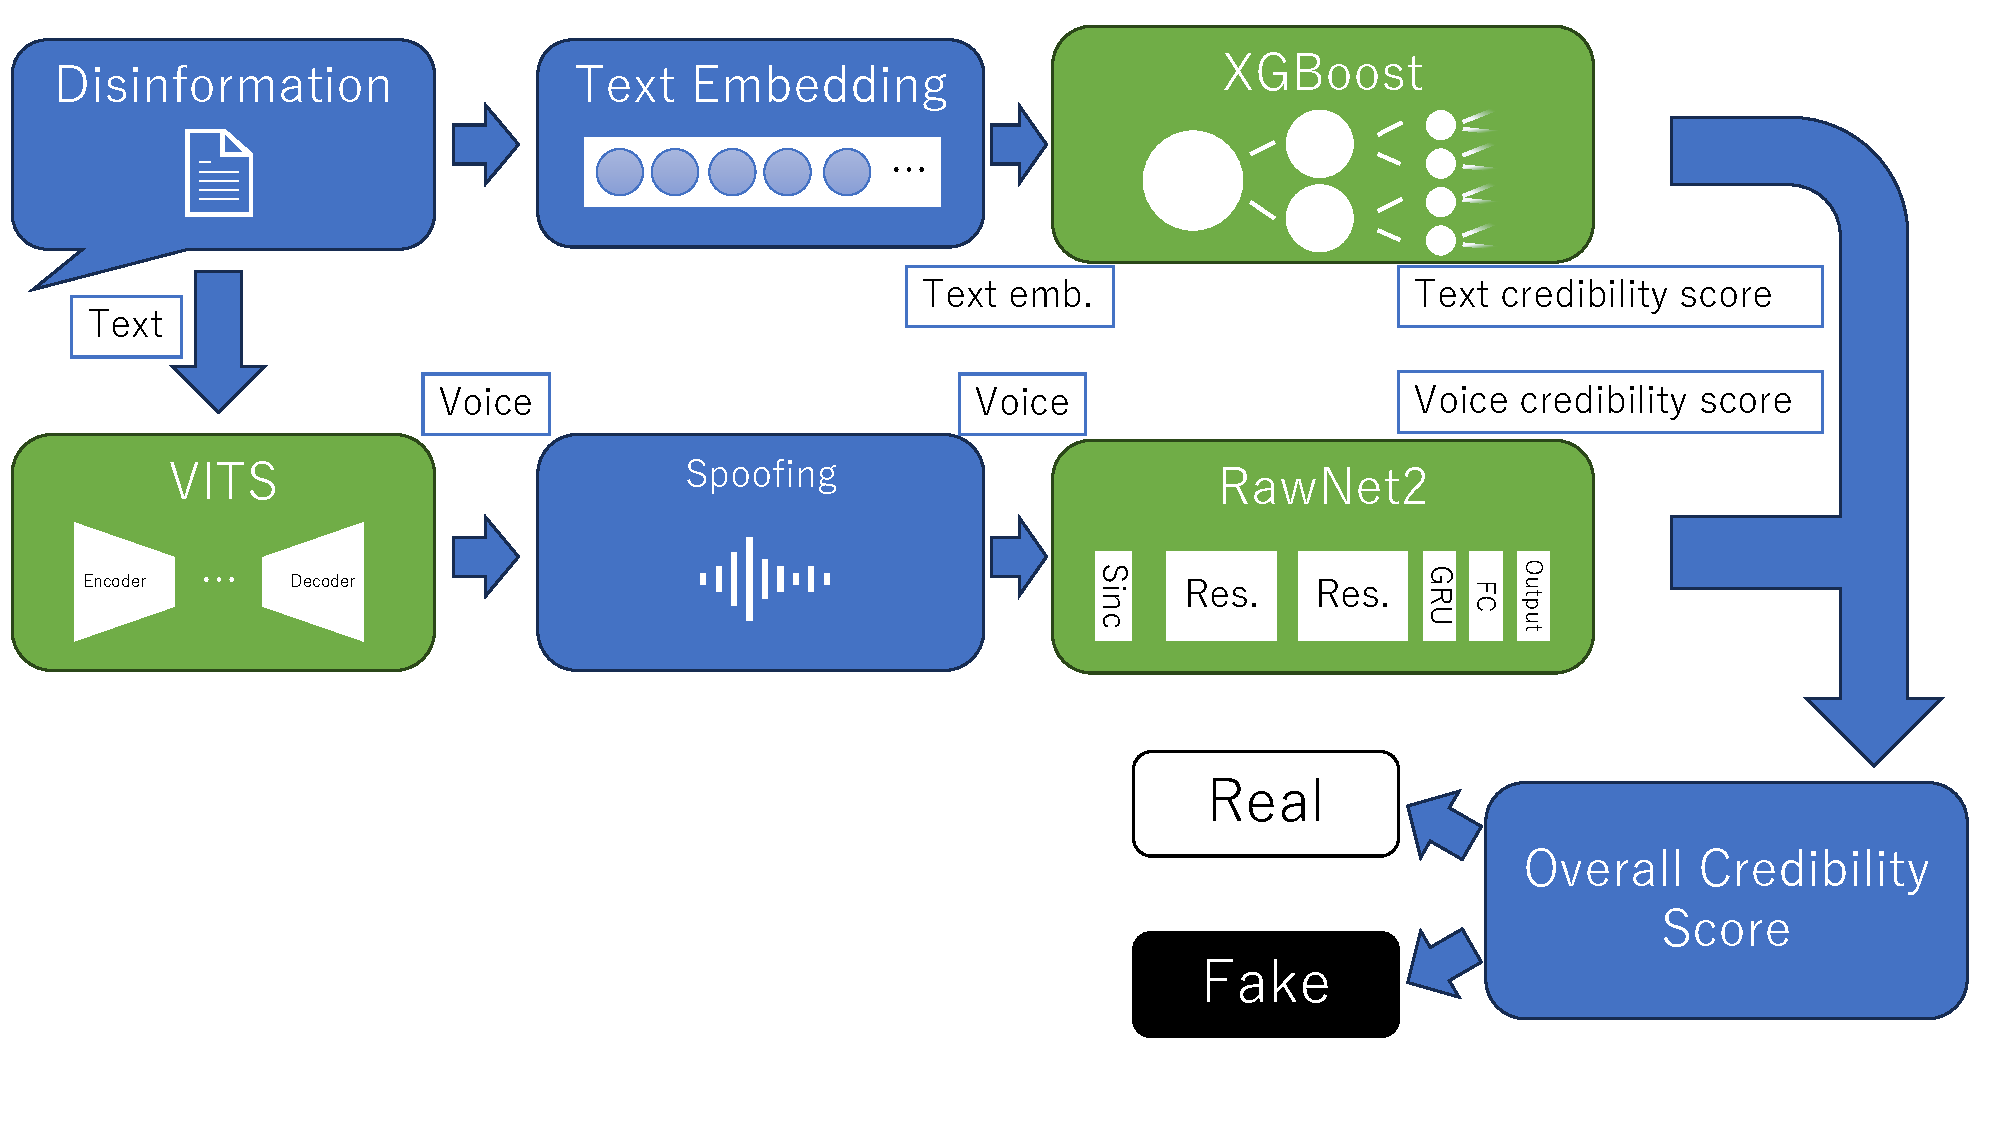
\includegraphics[width=\linewidth]{figures/Structure.pdf}
    \caption{データセットの生成から提案手法が行う分析の流れ。}
    \label{fig:structure}
\end{figure}

\subsection{波形分析}
偽音声の波形を直接分析するモデルとして、RawNet2とRawBoost、そしてSSL-Antispoofingを採用した。

\subsubsection{RawNet2}
音声波形を直接扱う既存手法として、
ASVspoofにてベースラインとして提供された \cite{WANG2020101114}RawNet2を採用した。
RawNet2はもともとRawNet \cite{jung19b_interspeech}から拡張された手法で、
いずれも発話レベルの特徴抽出と特徴拡張を単一モデルで完結させた上で分類を行う。
今回採用したRawNet2の構造は\cref{tb:rawnet2}の通りである。

RawNet2はRawNetモデル \cite{jung19b_interspeech}の拡張版である。
どちらのモデルも直接波形を分析して合成音声の疑いの強さを出力とするEnd-to-endの分類器として動作する \cite{jung19b_interspeech}。
RawNet2のフレームワークの最初のレイヤーは、SincNet \cite{8639585,ravanelli19_interspeech}として導入されたSinc-convolutionレイヤーを利用している。
SincNetは畳み込みニューラルネットワーク(CNN)を採用し、sinc関数に似たバンドパスフィルターを用いて入力波形をフィルターする。
第2層は残差ブロックからなり、バッチ正規化(BN)、LeakyReLU \cite{maas2013rectifier}、畳み込み層、最大値プーリング、特徴マップスケーリング(Feature Map Scaling, FMS)を含む。
FMSは \cite{woo2018cbam}で提案され、シグモイド活性化 \cite{jung20c_interspeech}を持つ注意層と同様の機能を持つ。
出力層は二値分類用に設計されており、合成によるなりすました音声と本人の音声を区別する。
このモデルは、GitHub リポジトリにある ASVspoof のベースライン設定に従って、重み付けされたカテゴリ横断エントロピーを損失関数として利用する。
これは本物の声と偽物の声を区別するための二値分類タスクであることから、本モデルの損失 $ L_{RN} $は以下の式で決定される。

\begin{equation}
    L_{RN}(y, \hat{y}) = -0.1 * y \log{\hat{y}} - 0.9 * (1-y) \log{(1-\hat{y})}
\end{equation}

この式では、$y$はラベルの値であり、$y=0$は本人に、$y=1$はなりすまし偽音声に該当する。
$\hat{y}$はRawNet2による出力に該当し、log関数にかけられている。
定数0.1及び0.9はASVspoof内での学習におけるラベル分布を根拠とする重み付けとして設定されている \cite{yamagishi21_asvspoof}。

%\begin{figure}[ht]
%    \centering
%    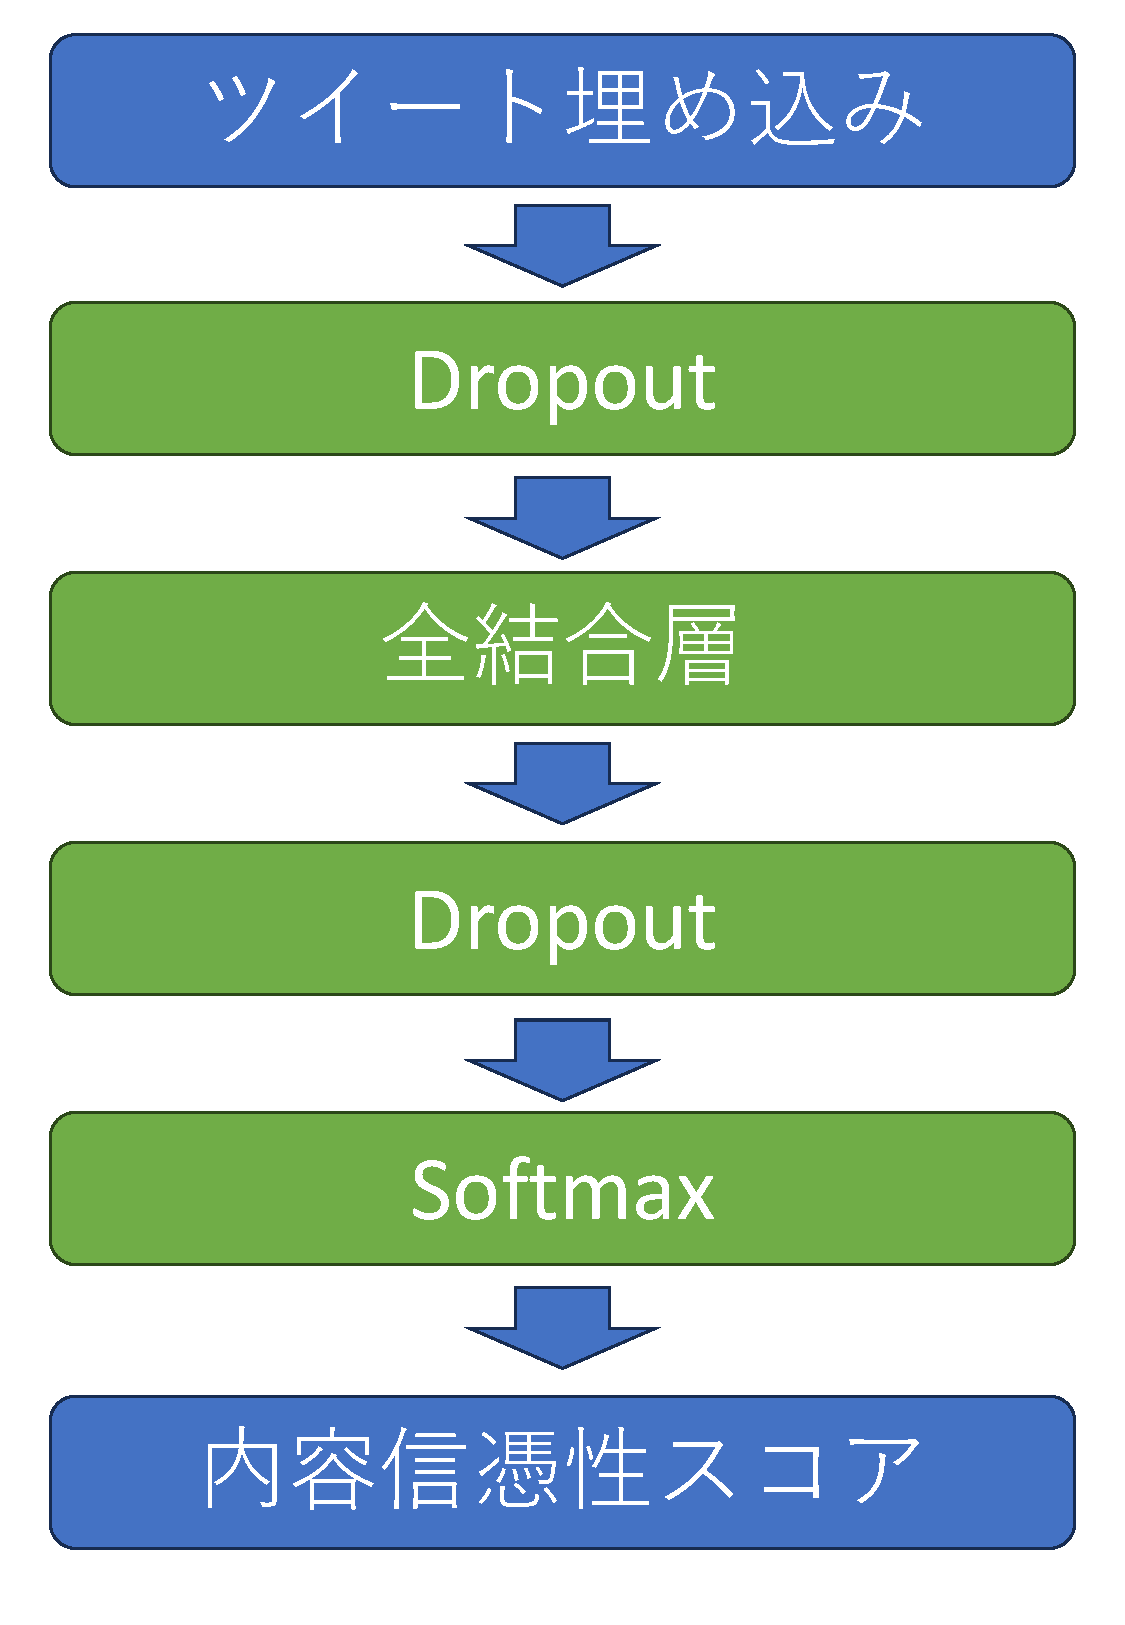
\includegraphics[width=0.5\textwidth]{./figures/ieice_nnfig.pdf} %TODO 次元情報追加
%    \caption{提案手法における内容信憑性評価部分。}
%    \label{fig:content}
%\end{figure}

\begin{table}[h]
    \centering
    \caption{ASVspoof 2019以降で採用されている \cite{9414234,yamagishi21_asvspoof}RawNet2の構造}
    \begin{tabular}{l@{}c@{}l}\hline
        層 & 入力 & 出力形式 \\\hline\hline
        \multirow{3}{*}{調整済Sincフィルタ} & 畳み込み(129,1,128) & \multirow{3}{*}{(21290, 128)}\\
        & 最大値プーリング(3) &\\
        & バッチ正規化(BN) \& LeakyReLU &\\\hline
        \multirow{6}{*}{残差ブロック}&\multirow{6}{*}{$\left\{\begin{array}{c}\rm{BN \& LeakyReLU}\\
        \rm{畳み込み(3,1,128)}\\
        \rm{BN \& LeakyReLU}\\
        \rm{畳み込み(3,1,128)}\\
        \rm{最大値プーリング(3)}\\
        \rm{特徴マップスケーリング(FMS)}\\\end{array}\right\}$}& \multirow{6}{*}{(2365, 128)}\\ \\ \\ \\ \\ \\\hline
        \multirow{6}{*}{残差ブロック}&\multirow{6}{*}{$\left\{\begin{array}{c}\rm{BN \& LeakyReLU}\\
        \rm{畳み込み(3,1,128)}\\
        \rm{BN \& LeakyReLU}\\
        \rm{畳み込み(3,1,128)}\\
        \rm{最大値プーリング(3)}\\
        \rm{FMS}\\\end{array}\right\}$}& \multirow{6}{*}{(29, 512)}\\ \\ \\ \\ \\ \\\hline
        ゲート付き回帰型ユニット&GRU(1024)&(1024)\\\hline
        全結合層&1024&(1024)\\\hline
        Output&1024&2\\\hline
        %& Maxpooling(3) &\\
    \end{tabular}
    \label{tb:rawnet2}
\end{table}

\subsubsection{RawBoost}
さらに、RawNet2とは別の手法としてRawBoost \cite{9746213}を採用した。
RawBoostは、学習にて音声内のノイズ対策として独自のデータ拡張手法を取り入れている \cite{9746213}。
このモデルを使用したのは、ASVspoofにおけるRawNet2を含むベースラインよりも良好なスコアが \cite{9746213}にて報告されたためである。
具体的なデータ拡張として、
(1)線形および非線形の畳み込みノイズ(符号化、圧縮、および送信プロセス中に導入されるノイズを再現している)、
(2)クリッピングやデバイス(マイクやアンプなど)の非最適動作などのインパルス信号依存の付加ノイズ、
(3)単一の有限インパルス応答フィルタを適用することによる定常信号非依存のノイズ付加
の3種類が導入されている \cite{9746213}。
さらに、学習時の損失関数として、GitHubリポジトリ \footnote{\url{https://github.com/TakHemlata/RawBoost-antispoofing}}で提供されている仕様に従って、同じ重み付きクロスエントロピー損失を採用した。

\subsubsection{SSL Anti-spoofing}
本実験では、SSL Anti-spoofingも導入した。
RawBoostと同じくTakら \cite{tak2022automatic}によって提案された手法である。
RawNet2との違いとして、入力を直接受ける部分がSincフィルタではなくwav2vec 2.0 \cite{NEURIPS2020_92d1e1eb}を導入し、自己教師あり学習を取り入れている。

この手法はASVspoof2021の開催後に行われた事後タスクにて参加シナリオ中で最も優秀な成績を収めている \cite{10155166}。

\subsection{埋め込みによる発話内容の分析}
音声の内容を考慮するために、MuMiNデータセット \cite{10.1145/3477495.3531744,NielsenMcConville2022}から得られる投稿埋め込みを活用する。
採用した理由として、データセット内でテキスト埋め込みが特徴としてすぐに使える点が挙げられる。
この埋め込みはBART-large-CNN \cite{lewis-etal-2020-bart}を使って生成される。
投稿埋め込み用の分類器としてXGBoost \cite{10.1145/2939672.2939785}を採用した。
今後の計画には、ディープニューラルネットワークモデルを組み込むことが含まれている。
また、自動音声認識モデルを統合し、ソーシャ ルメディアのコンテキスト内でDeep Fakeの声を検出する包括的なアプローチを取り入れることも視野に入れている。
損失$L_{emb}$は、Chen Tら \cite{10.1145/2939672.2939785}で詳しく説明されているように、重み付き二乗損失の平均として計算され、以下のように定義される。

\begin{align} 
        L_{emb} = \sum_l (\hat{y_i}, y_i) + \sum_k \Omega (f_k) \\
        \text{where}~\Omega (f) = \gamma T + \frac{1}{2} \lambda ||w||^2
\end{align}

この式では、$y_i$は$i$番目のラベルの値を示し、$\Omega$は葉ノードの数($T$)と重みのL2ノルムからなり、正則化項として総和がモデルの複雑さにペナルティを与える \cite{10.1145/2939672.2939785}。
定数$\gamma$および$\lambda$は今回では公式ドキュメント \footnote{\url{https://xgboost.readthedocs.io/en/stable/parameter.html}}にてモデルのデフォルト値とされていた0として実装した。
つまり今回では発話内容学習による損失は、事実上重みづけ二乗平均として算出される。
パラメータチューニングによる最適化は今後の手法改善における余地となっている。

\subsection{波形と内容検証結果の統合}
最終的な音声信憑性スコア$c_f$は波形および内容における検証結果スコアの平均によって導かれる。

\begin{equation}
    c_f = \alpha c_w + (1 - \alpha) c_{emb}
\end{equation}

$\alpha$は$[0, 1]$の範囲であり、波形分析による信憑性 $c_w$とテキスト埋め込みの分析による信憑性$c_{emb}$に対する係数として作用する。
$c_w$は波形分析を行うRawNet2の最終的な出力から $[0,1]$の範囲で正規化がなされている。

後述の波形分析単体で行う実験では $\alpha = 1$として扱ったほか、
実際に内容も考慮して検出を行う実験では $\alpha = 0.5$とした。
この判断は、SNSにおける偽情報を話すなりすまし偽音声を検出するための新しいアプローチを提示するという、我々の主要な目的と一致する。
確かにRawNet2の平均スコアとディープニューラルネットワークを介したテキスト埋め込みを統合する代替アプローチも考えられるが、この方法はかなりの計算資源と時間を必要とする。
即時性が求められるSNS環境における現実的なシナリオを考慮し、我々は効率性を重視するため、加重二乗損失の平均値のみに基づいて損失を計算する。

\section{予備実験: 既存手法における新型音声合成手法への対応}
提案手法の効果を測定する前に、既存の波形分析のみを行う手法が直近に提案された音声合成手法に対してどこまで検出精度を維持できるか実験を行った。

\subsection{データセット作成手法}\label{ssc:spc_ds}
音声波形に加えて発話内容を入力とする形で分類させるため、
事実に基づく情報を読み上げる音声と事実と異なる偽情報を読み上げる音声を用意した。
読み上げる対象はMuMiNデータセットが保有する英語の偽情報投稿とした \cite{10.1145/3477495.3531744}。
選定理由は、データセットから投稿文章とともに内容を埋め込みに変換した情報も得られることで、後述の提案手法への接続が容易に実現できるためである。
また、偽情報を扱うデータセットにはトピックや扱う属性の偏りに起因する情報の特殊性・バイアスが指摘されている \cite{10.1145/3477495.3531816}が、本データセットは政治・芸能・軍事・スポーツ・医療(COVID-19を含む)と多岐にわたる点も理由に含まれる。

Text-To-Speech(TTS)による読み上げ手法はVITSを採用した \cite{pmlr-v139-kim21f}。
\cref{ch:rel_res}で紹介した文章から音声を生成するText-To-Speechの形式であることと、
生成性能が良好である点が示されている点、
そして音声生成学習においてLJSpeechデータセット \cite{ljspeech17}による事前学習済みモデルが公開されており、生成への活用が容易である点から採用した。

なお実験で使用するにあたって、SNS上での投稿を想定して音声が3分以内に収まるように
英単語数の上限を480に設定し、超過分は切除した上でVITSによる音声生成を行った。
もっとも、$\mathbb{X}$の投稿は仕様上480文字までの制限があるため、今回実験で使用した音声長は最長でも24秒である。
データセットの統計は\cref{tb:dataset}の通りである。

\begin{table}[h]
    \centering
    \caption{実験で使用した偽音声データセットの統計}
    \begin{tabular}{lc}\hline
        項目 & 値\\\hline\hline
        投稿件数 & 722\\
        最大単語数 & 50\\
        平均単語数 & 24.9\\
        平均音声長 [\si{s}] & 8.2\\\hline
    \end{tabular}
    \label{tb:dataset}
\end{table}

\subsection{実験内容}
実験における環境は\ref{tab:env}の通りである。
今回は、RawNet2とRawBoostの2手法を検出モデルとして使用した。
これら2手法とも、ASVspoof 2021のDeep Fake(DF)タスクに使用されたモデルである。
RawNet2はDFのベースライン手法として提供がされ \cite{yamagishi21_asvspoof}、
RawBoostはDFタスクに実際に参加した手法の1つである \cite{9746213}。
また、両手法ともASVspoof 2021 DFデータセットを使用してトレーニングを行った。
具体的な学習は各手法の提案論文 \cite{9414234,9746213}にて詳細な学習プロセスが記述されている。
我々はGitHub \footnote{\url{https://github.com/asvspoof-challenge/2021/tree/main/DF/Baseline-RawNet2}}, 
\footnote{\url{https://github.com/TakHemlata/RawBoost-antispoofing}}
から事前学習済みモデルを入手した。
それぞれの検出モデルが、VITSによって生成させた音声データセットのうち何割を正しく偽音声と検出できたか調べた。

\begin{table}[h]
    \centering
    \begin{tabular}{lc} \hline
        事項 & 詳細 \\ \hline \hline
        CPUs & Intel\textsuperscript{\tiny\textregistered} Xeon\textsuperscript{\tiny\textregistered} CPU E5-2698 v4 @ 2.20GHz\\
        GPUs & TeslaV100-PCIE-32GB x8\\
        RAM & 503GB\\
        ROM & 7TB\\
        CUDAバージョン & 11.4\\
        フレームワーク & Python 3.10.8, PyTorch 2.1.0\\ \hline
    \end{tabular}
    \caption{実験環境。}
    \label{tab:env}
\end{table}

評価指標として、等価エラー率(Equal Error Rate, EER)を採用した。
本指標は本人拒否率(False Rejection Rate, FRR)と他人受入率(False Acceptance Rate, FAR)が同値になるよう閾値を調整した際の誤り率である。
EERはASVspoof 2021 DFにて導入されている唯一の評価指標である \cite{10155166}。
EERは以下の式によって算出される。

\begin{align}
    FRR = \frac{FN}{FN+TP}\\
    FAR = \frac{FP}{FP+TN}
\end{align}

本研究の文脈では、TP(True Positive)は、モデルが合成された偽音声を偽音声として正しく分類した場合を示す。
FN (False Negative) は、モデルが偽音声を本物の音声として誤って分類した場合を示す。
FP (False Positive) は、モデルが本物の音声を偽音声と誤って分類した場合を示す。
これらの定義は、本物の声と合成された声を区別する検出モデルの精度と有効性を評価するために不可欠な要素である。
この式によって、検出モデルのFRRとFARのバランスを最適化する閾値を決定することができる。

続いて、本研究で作成した音声データセットを用いて既存手法による出力をチェックした。
まずASVspoof 2021 DFデータセット \cite{10155166}のテストセットの出力において、EERが求まる条件に基づいて設定された閾値を取得した。
その後、本研究における開発データセットからの出力のうち何割がASVspoofによる閾値を上回ったかを評価した。
本研究の提案するデータセットが合成音声のみで構成されていることを考慮すると、これらの閾値を超えた事例の割合は合成音声の再現率を表す。

\subsection{結果}
\cref{tab:eer}、\cref{tab:preOut}、\cref{fig:hist}に予備実験の結果を示す。
\cref{tab:eer}はモデルのEER値と検出に使用される閾値を示している。
モデルの出力は、信憑性を決定する上で重要な役割を果たす。
出力が閾値を超えると、そのモデルは入力音声を偽物として識別したことを意味する。
つまり、閾値の調整はモデルのパフォーマンスに大きな影響を与える。
閾値を低い値に設定すると、モデルはより敏感になり、より多くの偽の音声を検出することができる。
しかし、これは偽陽性の増加につながる可能性があり、本物の声が誤って偽の声として分類されてしまう。
逆に、閾値を高く設定すると、モデルの感度が低くなり、誤検出の可能性が低下する。
その一方で、偽の音声が検出されないなど、なりすましの影響を受けやすくなる。
前節の通り、最適な閾値を決定するために、ASVspoof 2021 DF データセットを利用した。
このデータセット内でEERが求まる条件における閾値を選択した。

\begin{table}[h]
    \centering
    \begin{tabular}{lcc}\hline
        モデル名 & RawNet2 & RawBoost \\ \hline \hline
        等価エラー率 (EER) [\%] & 25.5 & 81.0 \\
        EER算出時の閾値 & -5.74 & $2.77 * 10^-6$ \\ \hline
    \end{tabular}
    \caption{ASVspoof 2021 DFデータセットに対する分類モデルのEERおよび閾値。RawNet2の出力はLogSoftmax関数を使用して生成され、出力値は$(-\inf,0)$の範囲内になる。出力値が高いほど、入力音声が偽物である可能性が高いことを示す。入力が偽音声かどうかを判断するには、閾値を設定する必要がある。}
    \label{tab:eer}
\end{table}

\begin{table}[h]
    \centering
    \begin{tabular}{lccc} \hline
        データセット & 指標 & RawNet2 & RawBoost \\\hline \hline
         & 最小 & -9.11 & $2.77 * 10^-7$ \\
        \multirow{2}{*}{ASVspoof 2021 DF} & 最大 & 0.00 & 1.00 \\
         & 平均 & -6.31 & 0.06 \\
         & 中央 & -7.57 & $1.02 * 10^-6$ \\ \hline
         & 最小 & -8.670 & $1.50 * 10^-7$ \\
         \multirow{2}{*}{MuMiN内の偽情報 + VITSによる偽音声}& 最大 & 0.00 & 1.00 \\
         & 平均 & -7.88 & $2.30 * 10^-3$ \\
         & 中央 & -8.05 & $1.05 * 10^-6$ \\ \hline
    \end{tabular}
    \caption{予備実験における、ASVspoofおよび本研究にて作成した偽音声データセットに対する既存手法による出力値の傾向。出力値は事実上「疑わしさ」として扱うことができる。}
    \label{tab:preOut}
\end{table}

\begin{table}[h]
    \centering
    \begin{tabular}{lcc}\hline
        モデル名 & RawNet2 & RawBoost \\ \hline \hline
        閾値を上回った偽音声数 & 5 & 32 \\
        入力数に対する割合[\%] & 1.08 & 6.88 \\ \hline
    \end{tabular}
    \caption{本研究にて作成したVITSによる偽音声を入力とした際の、出力値が閾値を上回った偽音声の数。これらの閾値は、ASVspoof 2021 DFの出力からEERの計算時に設定された値に対応する。}
    \label{tab:greater}
\end{table}

\begin{figure}
    \centering
    \begin{minipage}[b]{0.45\hsize}
        \centering
        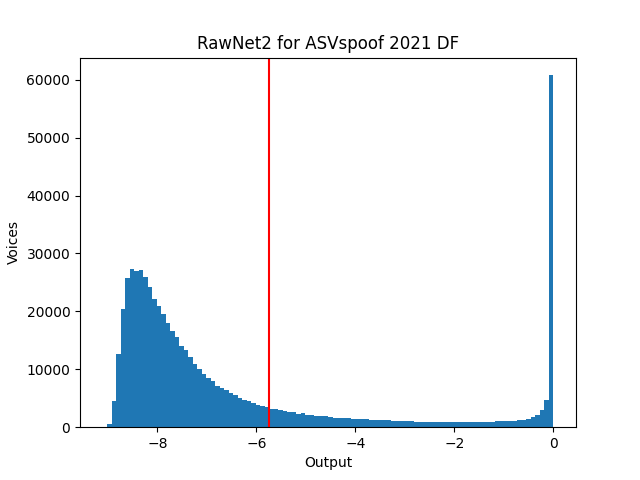
\includegraphics[width=\linewidth]{figures/rawnet2_asv.png} 
        \subcaption{}
    \end{minipage}
    \begin{minipage}[b]{0.45\hsize}
        \centering
        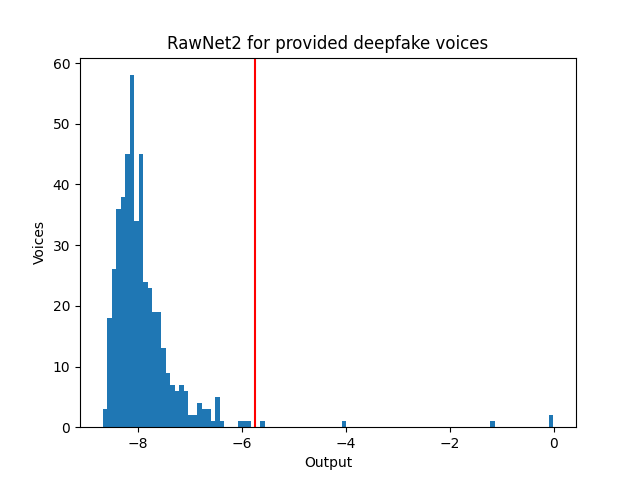
\includegraphics[width=\linewidth]{figures/rawnet2_prop.png}
        \subcaption{}
    \end{minipage}\\
    \begin{minipage}[b]{0.45\hsize}
        \centering
        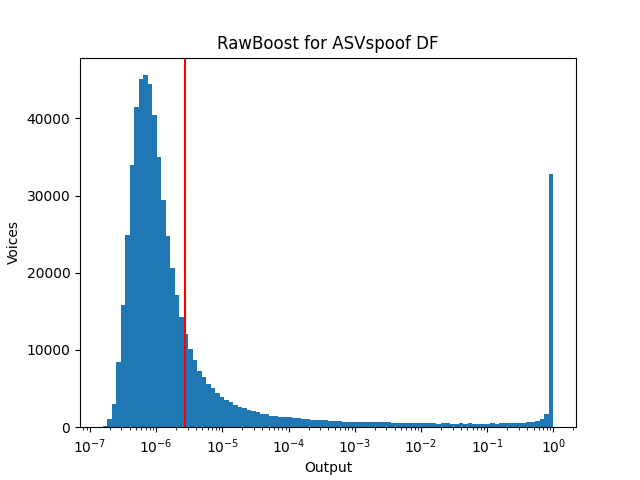
\includegraphics[width=\linewidth]{figures/rawboost_asv.png} 
        \subcaption{}
    \end{minipage}
    \begin{minipage}[b]{0.45\hsize}
        \centering
        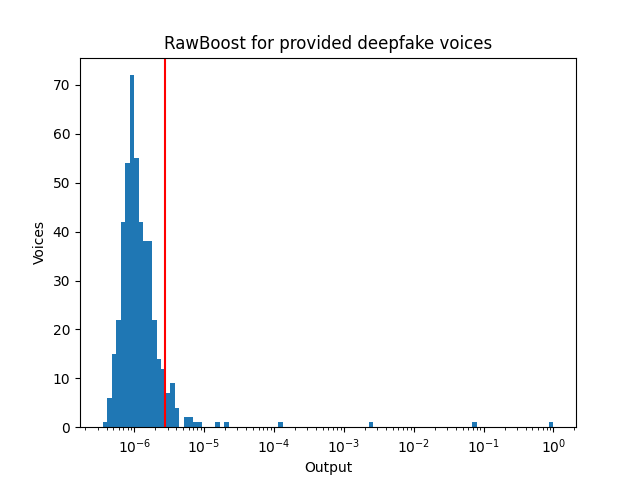
\includegraphics[width=\linewidth]{figures/rawboost_prop.png}
        \subcaption{}
    \end{minipage}
    \caption{モデルおよび使用データセット毎の出力値のヒストグラム。(a)ASVspoof2021DFに対するRawNet2、(b)提案偽情報データセットに対するRawNet2、(c)ASVspoofのRawBoost、(d)提供データセットのRawBoost。赤い線はASVspoofデータセット内のEERの状況に合わせた閾値を表す。}
    \label{fig:hist}
\end{figure}

また、RawNet2 の閾値が負の値であることに注意することが重要である。
これはLogSoftmax関数を適用するモデルの仕様の影響で、RawNet2の出力が常にゼロか負であるためである。
RawNet2の場合、その性能は\cite{yamagishi21_asvspoof}によるASVspoof 2021の記事で報告された結果と密接に一致する。
しかし、RawBoostに関しては、ASVspoof DFタスクでのパフォーマンスはRawNet2を下回る成績だった。
この傾向は、RawBoostが当初この特定のタスクのために設計されたものではなかったことに起因している可能性がある。
提案したデータセットからの出力値の適用を標準化するために、ASVspoof DFデータセットのEERから導き出した閾値を採用した。
このアプローチにより、異なるモデルやデータセット間で一貫性のある比較ができた。

\cref{tab:preOut}にモデルの出力値を示す。
両モデルに共通する特徴は、出力値が音声に関連する疑いのレベルを反映していることである。
ASVspoof データセットの結果に基づき、ASVspoof データセットの EER で設定された閾値を超える値は、偽音声が疑われると本研究の実験では解釈する。
\cref{fig:hist}に示すように、ASVspoof データセットと比較すると、本研究の提供する音声は、偽音声として検出された割合が大幅に低下している。
この結果は、予備実験のデータセットが主に合成音声で構成され、実際に検出された音声は 1つしか含まれていないことを考えると、重大な懸念事項である。
同様の傾向は、\cref{tab:preOut} の平均値と中央値を調べたときにも明らかであり、本研究が提供した音声の平均値と中央値は、ASVspoof 2021 DF タスクで観察された値よりも著しく小さい。
さらなる分析として、\cref{tab:greater}に出力が閾値を超えた偽音声の数を示す。
ASVspoofデータセットが閾値を設定し、出力値がこの閾値を超えた場合、その音声はDeepFakeとして識別される。
RawNet2では5つの音声が偽音声として検出され、RawBoostでは32の音声が偽として検出された。
ただし、RawBoost は EER が低いため、結果の信頼性には疑問が残ることに留意が必要である。
この結果はどちらのモデルも、提供されたデータセットの全サンプルの 10\%未満しか偽音声として識別していないことを示す。
さらに、生成された音声を聴いたところ、明らかな偽音声として判別できるような目立ったアーティファクトや不自然な点は確認できなかった。
まとめると、どちらのモデルも入力音声を偽音声ではなく本物であると判断していた。


\section{本実験: 波形・内容の2面による検出性能の検証}\label{sec:cnt_main}
本実験では、波形と発話内容を考慮して、新たに提案したフレームワークを検証した。
環境は、\ref{tab:env}が示すように、予備実験と同じ条件である。

\subsection{データセット}
本実験では、提案モデルにおいて、事実と偽の主張を伝える合成音声を含む別のデータセットを作成した。
この新しいデータセットは二値ラベルを採用し、合成音声を「事実」と「偽情報」の2クラスに分類する。
今回の文脈では、「事実」(``factual'')ラベルは事実を報じるニュースを伝える合成音声に割り当てられ、偽情報(``misinformation'')ラベルは偽情報を広める合成音声に該当する。
この2ラベルはMuMiN内での記載ラベル名に由来するものである。
本来\cref{ch:background}の通り``misinformation'' は誤報という定義に該当するが、MuMiNが保有する該当投稿の殆どが偽情報の定義にも該当するため、本研究では偽情報として扱う。
予備実験と本実験の顕著な違いの一つは、データセット内の事実と偽の主張の比率である。MuMiN-largeデータセットでは、英語の投稿8,013件を保有する。
しかしながら、事実を示す投稿は357件にとどまる。
この不均衡に対処するため、偽情報の数を意図的に減らし、事実の主張の量に近づけた。
全投稿数は723で、357の事実投稿と365の偽情報投稿である。
また、音声生成のための前処理として、すべての投稿からURLと絵文字を削除した。
本実験で使用した合成音声は、VITSモデルを利用し、予備実験と同じ条件でデータセットから取得した。
実験と評価を容易にするため、このデータセットをトレーニングセット、検証セット、テストセットに0.7/0.1/0.2の割合で分割し、学習およびテストを行った。

\subsection{実験内容}
この実験では、主張の信憑性を評価する要素の重要性を調査した。
その実現に向け、波形と音声コンテンツの両方を考慮する新しいフレームワークを評価した。
さらに、実験に必要な事実と捏造の主張に関連する合成音声を含むデータセットを導入した。

提案するフレームワークモデルの波形セクションでは、RawNet2を採用した。
モデルの設定を維持したまま、微調整なしで音声波形データを入力した。
その後、出力を0から1の範囲で正規化し、波形の疑わしさを表現した。
発話内容評価では、MuMiNデータセットから取得した投稿の埋め込みを利用した。
学習データセットの埋め込みに対してXGBoost分類器を訓練した。
最後に、提案するフレームワークの波形とコンテンツの両コンポーネントからの出力の平均を計算した。
最終出力は音声に関連する疑わしさの度合いを示している。
EERと正確性(Accuracy)に基づき、提案フレームワークモデルを波形のみ・コンテンツのみのモデルを含む単一ユニットモデルと比較した。 
また、ASVspoof 2019のLAセットでRawNet2の性能を確認し、このモデルが従来の手法で偽音声を正確に検出できる点を証明することを意図した。
EERを使用したのは、これがASVspoof 2021 DFの評価指標であったためである。
MuMiN+VITSによる音声セットやASVspoof 2019 LAセットの結果と比較するためにAccuracyを採用した。
これは、ASVspoof 2019 LAセットには事実のニューステキストしか含まれていないためである。
具体的には、EERの算出に必要な値であるTrue PositiveとFalse Negativeが不足しているため、コンテンツのみではASVspoofデータセットのEERを得ることができない。
そのため、別の指標であるAccuracyを設定した。
なお、本実験における波形単体も含めた全モデルにおける正誤は予備実験とは異なり、内容の偽・真を判定対象としている。
これは、本実験においては事実を話す合成音声と偽情報を話す合成音声で実験しているためである。
本実験では$y=0$は事実を話す本人音声を示し、$y=1$は偽情報を話す合成音声としてラベル付け及び学習を行っている。

また、本実験ではSSL Anti-spoofingのMuMiN+VITSデータセットに対するパフォーマンスも確認した。
このモデルは、ASVspoof 2021 DF post-challenge \cite{10155166}の参加者の中で、最高のパフォーマンスを発揮していたことから、本実験で採用した。

\subsection{結果}\label{sec:cnt_res}
本実験では、モデルが偽情報を主張する合成音声を識別できるかどうかを検証した。
この本実験の結果を\ref{tab:result}に示す。
波形のみのモデルで情報の真偽を分類した場合、EER は44\%で、accuracyは50\%に近く、ランダム選択に近い結果を示した。
この結果は、偽音声を波形のみの観点から検出するモデルの能力が限定的であることを浮き彫りにしている。
一方で、本研究が提案する波形と内容を考慮したモデルが最も優れていることが示された。

また、ASVspoof 2019 LAセットに対してRawNet2が正確に分類された点も確認した。
この分類は本人かそうでないかの2カテゴリ分類であり、
この結果はTakらの報告 \cite{9414234}を支持するものである。
SSL anti-spoofingの結果は、ASVspoofの結果において、他のモデルからの改善を示している。
この結果もASVspoof 2021の報告 \cite{10155166}を支持するものである。
しかし、MuMiN+VITSのデータセットにおけるEERは54\%であり、他波形単独手法と同様にまだ改善の余地がある。
この部分からも、波形のみで偽情報を話す偽音声を検出することは、最新の音声生成モデルでは不十分であることが示唆される。
また、これら2つのデータセットの平均値から、SSL anti-spoofingを含む比較モデルの中で、提案手法が最も精度の高い性能を示した。
この結果は、提案フレームワークは実際のSNS上での運用において最新の音声生成モデルと効果的に対応できることを示唆している。

% \begin{landscape}
% \begin{table}[h]
%     \caption{事実に基づく情報と、事実と異なる偽情報を話す合成音声を真偽分類した結果。(*)は、データセットに偽情報記事が含まれていないため、計算不可能な値であることを示す。}
%     \centering
%     \begin{tabular}{lcc|ccc}\hline
%          & \multicolumn{2}{c}{等価エラー率 [\%]} & \multicolumn{3}{c}{accuracy [\%]}\\
%        モデル形式 & MuMiN + VITS & ASVspoof 2019 LA & MuMiN & ASVspoof & 平均\\\hline\hline
%        波形のみ(RawNet2) & 44.6 & 5.6 & 52.7 & 99.7 & 76.2\\
%        波形のみ(SSL anti-spoofing) & 54.1 & 2.9 & 46.3 & 99.8 & 73.1\\\hline
%        内容のみ(埋め込み+XGBoost) & 32.4 & \multirow{2}{*}{N/A*} & 86.8 & 11.5 & 49.2\\
%        提案手法: 波形+内容 & 17.6 & & 81.7 & 81.6 & 81.7 \\\hline
%     \end{tabular}
%     \label{tab:result}
% \end{table}
% \end{landscape}

% \begin{landscape}
\begin{table}[h]
    \caption{事実に基づく情報と、事実と異なる偽情報を話す合成音声を真偽分類した結果。(*)は、データセットに偽情報記事が含まれていないため、計算不可能な値であることを示す。}
    \centering
    \begin{tabular}{lccc}\hline
         & \multicolumn{3}{c}{等価エラー率 [\%]} \\
       モデル形式 & MuMiN + VITS & ASVspoof 2019 LA \\\hline\hline
       波形のみ(RawNet2) & 44.6 & 5.6 & \\
       波形のみ(SSL anti-spoofing) & 54.1 & 2.9 & \\\hline
       内容のみ(埋め込み+XGBoost) & 32.4 & \multirow{2}{*}{N/A*} & \\
       提案手法: 波形+内容 & 17.6 & &\\\hline\hline
       & \multicolumn{3}{c}{Accuracy [\%]}\\
       & MuMiN & ASVspoof & 平均\\\hline
       波形のみ(RawNet2) & 52.7 & 99.7 & 76.2\\
       波形のみ(SSL anti-spoofing) & 46.3 & 99.8 & 73.1 \\
       内容のみ(埋め込み+XGBoost) & 86.8 & 11.5 & 49.2\\
       提案手法: 波形+内容 & 81.7 & 81.6 & 81.7 \\\hline\hline
    \end{tabular}
    \label{tab:result}
\end{table}
% \end{landscape}

\section{考察}\label{sec:cnt_evl}
\subsection{音声合成と検出の発展速度差}
予備実験の\cref{tab:preOut}によると、音声生成の進歩に検出が追い付いていない点が重要な問題として浮上している。
ASVspoofでベースラインとして提供されたRawNet2は、RawBoostと同様に、最新のText-To-Speech(TTS)で合成された音声を正しく偽として検出できなかった。
この結果は、2019年以前のTTSとVCモデルを組み込んだデータセットで訓練されたモデルは、2020年以降に開発されたモデルに対応できないことを意味する。
注目すべきは、この性能低下はASVspoof 2021の報告 \cite{yamagishi21_asvspoof}で以前から認められていたことでもある。
一方で本研究は、2021年以降の方法に特化した音声合成の結果を提供するものであり、その間に大きな合成側の前進がある。
偽音声合成側の進歩が速いため、新しい波形分析方式による偽音声検出手法が提案されてから、良好な検出成績を長い期間提供できない可能性が考えられる。
これを裏付けるように、直近に提案された手法であるNaturalSpeech \cite{10409539} によって、対象人物の音声から生成した合成音声と本人音声とのコサイン類似度を測定したところ0.9前後と高く、予備実験と同じく検出は困難とみられている。

本実験の結果、\cref{tab:result}の各データセットの性能評価において、提案手法が最も優れていることが示された。
本実験は、波形に加えて発話内容の使用による進歩と改善点を確認することを目的としている。 
したがって、提案スコアは波形と内容において個々のモデルよりも優れており、この結果は我々のコンセプトの効果を証明している。

\subsection{提案手法の改善点}
我々の提案するフレームワークモデルは、現実のシナリオに適用した場合、顕著な改善を示している。
具体的には、SNS上に投稿された対象音声を我々のモデルに展開するシナリオを想定している。
この文脈では、投稿埋め込みを直接利用できないという課題に直面することに注意しなければならない。
この制限を克服するためには、音声認識モデルを採用して音声コンテンツをテキストに書き起こす必要がある。
最終的には、入力コンテンツが波形データのみで構成されている場合でも、
本研究の形式が効果的に音声を正確に分類できるようにする必要がある。

さらに、本人が偽情報を読む場合も想定し、合成音声と人間が録音した音声の両方を包含する追加データセットを作成する必要がある。
本稿では、提案モデルの偽の主張を検出する能力を評価することを主目的としたため、録音された音声を取り込まなかった。
本研究では今後録音された声と合成された声、そして事実と偽の内容という2つの観点を考慮した4クラス分類を含む別の実験も考えられる。